% =====================
% Main document
% ---------------------
% =====================

%!TEX TS-program = xelatex 
%!TEX encoding = UTF-8 Unicode

\documentclass[11pt, twoside, a4paper]{book}

\usepackage[pdftitle={The Bees Algorithm for the Vehicle Routing Problem},
pdfauthor={Aish Fenton},
]{hyperref}

% \usepackage{multirow} 

\usepackage[ruled]{algorithm2e}
\SetAlgoInsideSkip{smallskip}
\setlength{\interspacetitleruled}{4pt}

% \usepackage{epstopdf}

\usepackage{amssymb}
\usepackage{amsmath}
\usepackage{amsthm}

\usepackage{graphicx}
\usepackage{fontspec}
\usepackage{xltxtra}

% \setromanfont{Fontin-Regular}
% \setsansfont{Avenir LT Std}
% \setmonofont{Lucida Sans Typewriter}

% Gives more control over how figures are floated
\usepackage{float}

\usepackage{pdflscape}
\usepackage{ctable}

\widowpenalty=9000
\clubpenalty=9000

\textwidth      = 14.3cm
\textheight     = 22cm
\oddsidemargin  = 1.53cm
\evensidemargin = 0cm
% \topmargin      = 0.0in
% \headheight     = 0.0in
\parskip        = 0.2in
\parindent      = 0.0in
% \footskip       = 0.8in
\setlength{\skip\footins}{1cm}
\raggedbottom

% provides a nicer looking caption for figures
\usepackage[margin=40pt,font=small,format=plain,labelfont=bf,textfont=it]{caption}

% \usepackage{setspace}
% \singlespacing
% \onehalfspacing
% \doublespacing
% \setstretch{1.1}

% \renewcommand{\multirowsetup}{\centering}

% =====================
% ---------------------
% MACROS
% ---------------------

\newcommand{\FTL}{\mbox{FTL}}
\newcommand{\LTL}{\mbox{LTL}}
\newcommand{\PDPFTL}{\mbox{PDP-FTL}}
\newcommand{\CVRP}{\mbox{CVRP}}
\newcommand{\VRP}{\mbox{VRP}}
\newcommand{\MDVRP}{\mbox{MDVRP}}
\newcommand{\VRPTW}{\mbox{VRPTW}}
\newcommand{\PDP}{\mbox{PDP}}
\newcommand{\PDPTW}{\mbox{PDPTW}}
\newcommand{\DARP}{\mbox{DARP}}
\newcommand{\TSP}{\mbox{TSP}}
\newcommand{\MTSP}{\mbox{MTSP}}
\newcommand{\BPP}{\mbox{BPP}}
\newcommand{\schd}{\mathfrak{S}}

%!TEX root = main.tex

% =====================
% MACROS
% ---------------------
% =====================

%
% Required packages
%

\usepackage{color}

%
% Macros and theorems environments
%

% Environments
%
\newtheorem{lemma}{Lemma} 
\newtheorem{theorem}[lemma]{Theorem}
\newtheorem{conjecture}[lemma]{Conjecture}
\newtheorem{corollary}[lemma]{Corollary}

\theoremstyle{definition}
\newtheorem{case}{Case}
\newtheorem{definition}[lemma]{Definition}
\newtheorem{example}[lemma]{Example}

%\newtheorem{proof}{Proof}[lemma]

% Misc
%

\newcommand{\todo}[1] {
\fbox{#1}
}

\newcommand{\hquote}[1] {
\textcolor {blue}{#1}
}

% \newcommand{\comment}[1]{\fbox{#1}}

\newcommand{\mnote}[1]{\marginpar{%
      \vskip-\baselineskip
      \raggedright\footnotesize
      \itshape\hrule\smallskip\scriptsize{#1}\par\smallskip\hrule}}  
      
 
% Number families
%
\newcommand{\naturaln}{\mathbb{N}}

% Graph notation
%
\newcommand{\edge}[1]{(#1)}
% \newcommand{\edge}[2]{(#1#2)}
\newcommand{\isub}[2]{#1[#2]}

% Tree notation
%
\newcommand{\branchno}[1]{\ensuremath{\mathcal{B}(#1)}}


% Operator macros
%

% Family
\newcommand{\family}{\ensuremath{\mathcal{F}}}

% Running Time
%
\newcommand{\npcomplete}{$\cal NP$-complete}
\newcommand{\nphard}{$\cal NP$-hard}
\newcommand{\NP}{\mbox{$\cal{NP}$}}
\newcommand{\poly}{\mbox{$\cal{P}$}}
\newcommand{\BIGO}[1]{\mbox{$O(#1)$}}


% Logic
%
% \newcommand{\AND}{\wedge}
% \newcommand{\OR}{\vee}


% Set functions
%
\newcommand{\union}{\cup}

\newcommand{\bigunion}{\bigcup}

\newcommand{\intersect}{\cap}
\newcommand{\contract}[2]{#1/#2}
% \newcommand{\MIN}[1]{\mbox{$min(#1)$}}
% \newcommand{\MAX}[1]{\mbox{$max(#1)$}}
\newcommand{\set}[1]{\{#1\}}
\newcommand{\seq}[1]{[#1]}
\newcommand{\tuple}[1]{(#1)}
\newcommand{\PS}[1]{\ensuremath{\mathcal{P}(#1)}}
\newcommand{\compl}[1]{\overline{#1}}
\newcommand{\length}[1]{|#1|}


% Image functions
%
% \newcommand{\pic}[3]{\begin{figure}\begin{center}\includegraphics[scale=1.0]%
%  {#1}\caption{#2}\label{#3}\end{center}\end{figure}}

\newcommand{\picscl}[4]{\begin{figure}[htb]\begin{center}\includegraphics[scale=#4]%
	{#1}\caption{#2}\label{#3}\end{center}\end{figure}}

%------------------------
% Problems
%------------------------

\newcommand{\probdommin}{\mbox{DOMINATING SET}}
\newcommand{\probvertcov}{\mbox{VERTEX COVER}}
\newcommand{\probindset}{\mbox{INDEPENDENCE SET}}
\newcommand{\probhamcir}{\mbox{HAMILTONIAN CIRCUIT}}

%------------------------
% Logic
%------------------------
\renewcommand{\implies}{\Rightarrow}
% \newcommand{\equates}{\Leftrightarrow}



%------------------------
% Functions
%------------------------



%------------------------
% Specific Macros
%------------------------








% =====================
% ---------------------
% CONTENT
% ---------------------

\begin{document}

\pagestyle{empty}
\pagenumbering{roman}
%!TEX root = main.tex

% =====================
% TITLE PAGE
% ---------------------
% =====================

\pagestyle{empty}
% \fontspec{Gotham HTF Bold Italic}
% \addfontfeature{LetterSpace=5.0}

\LARGE
\begin{flushleft}
Meta-Heuristics for the Vehicle Routing Problem - \\[0.2Cm]
\hspace{1.0cm} Review and Case Study\\[0.2cm]
\end{flushleft}

\normalsize
\begin{flushleft}
Michael J. Dinneen \ Aisha J.L. Fenton
\end{flushleft}

\vfill
\rmfamily
\begin{flushright}
Department of Computer Science\\
University of Auckland \\
Auckland, New Zealand 
\end{flushright}

\cleardoublepage
%!TEX root = main.tex

% =====================
% PREFACE
% ---------------------
% =====================
\chapter*{Preface}

This MSc.~thesis has been prepared by Aisha Fenton at the University of Auckland---Department of Computer Science. It has been supervised by Dr.~Michael Dinneen. The work undertaken in this thesis has grown out of a research project sponsored by New Zealand Trade and Enterprise (NZTE) for the company vWorkApp Inc.~to research vehicle route optimisation for use within their software product.

\section*{Acknowledgements}

I'd like to thank my partner in crime, Anna Jobsis, for her encouragement, cajoling, threatening, bribing, doing the dishes, proof reading, guilt tripping, spellchecking... doing whatever it takes to help me get it done.

Thanks to Steve Taylor and Steve Harding for holding down the fort at work while I disappeared to do this thesis. And likewise thanks to my team, Jono, Rash, Elena, Bob, Marcus, Yuri, and Robin for being on the ball (as always) despite my absence.

Thanks to Brendon Petrich and vWorkApp Inc.~for providing me with time off work and being supportive of me undertaking this. 

And lastly, I especially owe Dr.~Michael Dinneen, my supervisor, a big thank you for persevering with me even though he must have doubted that I'd ever finish.

% =====================
% Abstract
% =====================
\cleardoublepage

\begin{center}
   \begin{minipage}{300pt}
   \begin{center}
      \textbf{Abstract}
   \end{center}
   In this thesis we present a new algorithm to solve the Vehicle Routing Problem. We adapt a fairly recent algorithm, the Bees Algorithm, which was developed for continuos problems, for use on the Vehicle Routing Problem. The results obtained are competitive with the best meta-heuristics available for the Vehicle Routing Problem. Additionally, the algorithm has good runtime performance, producing results within 2\% of the optimal solution within 60 seconds.
   \end{minipage}
\end{center}

\cleardoublepage


\pagenumbering{arabic}
\cleardoublepage
\tableofcontents

\pagestyle{headings}
%!TEX root = main.tex

% =====================
% Introduction Chapter
% =====================
\chapter{Introduction}

TODO


% =====================
% SECTION
% =====================
\section{Motivation}

% The VRP is an important combinatorial optimisation problem. Toth and Vigo  have 
% reported in 2002 (Maffioli 2003) that the use of computerised methods in distribution 
% processes often results in savings ranging from 5% to 20% in transportation costs. Barker 
% (2002) describe several case studies where the application of VRP algorithms has led to 
% substantial cost savings.
% In this paper the def


% =====================
% Sub Section
\subsection{Road transport industry}

% Road transport is a vital part of New Zealand. It is important for providing basic needs: virtually every product grown, made or used in New Zealand will be carried on a truck at least once during its lifetime\cite{RTFNZ}. And it is important for the New Zealand economy. The success of New Zealand's export industries are inextricably linked to the reliability and cost effectiveness of road transport.
% 
% New Zealand is inline with other countries in having 80\% of all freight transported by road (by comparison Europe also carries 80\% of all freight road). Road transport is particularly important to regional New Zealand and the export industries which drive these local economies. Trucks carry\cite{RTFNZ}:
% \begin{itemize}
%  \item 95\% of export fruit
%  \item 86\% of export wool
%  \item 85\% of export dairy products
%  \item 65\% of export logs
%  \item 35\% of export meat
% \end{itemize}
% 
% Road transport is a also very closely tied to the New Zealand economy. A study by \cite{?} showed that a 1\% growth in national output requires a 1.5\% increase in transport services.
% 
% In addition to this Road transport is itself a major contributor to the New Zealand economy. The road transport industry has a total turnover of around \$4 billion a year. This equates to around 1.4\% of economic activity nationally and goes as high as 2.5\% of economic activity in regional areas such as Southland\cite{RTFNZ}.

% XXX I'd love to be put this in but need to track down source
% A 2002 study by Infometrics found that a 10\% reduction in road transport freight rates would:
% 
% \begin{itemize}
% 	\item Create 33,000 new jobs
% 	\item Increase GDP by 3.7\%
% 	\item Boost exports by 3.9\% or more than \$1.5 billion
% \end{itemize}

% Most road transport business runs on tight margins \cite{NEED A CITE FOR THIS}. Therefore technology innovations are seen as key area for investment and as having a great potential for enabling the industry to grow. Technology research is focused on providing solutions in the following areas:
% \begin{itemize}
%  \item Improving fuel efficiency (e.g. improved engines, improved aerodynamics)
%  \item Reducing environmental impact of Road transport
%  \item Improving utilization of the fleet
%  \item Reducing running costs of a fleet
%  \item Strain on transport network. Limiting factor for economic growth.
% \end{itemize}
% 
% Improvements to vehicle routing has benefits in each of these areas. An optimal schedule will reduce the amount of distance travelled to perform the same amount of work, therefore it: reduces fuel costs, reduces environment impact as less work is required to move the same amount of freight, allows more good to be carried for the same cost, allows for more efficient use of the existing road network.  

% \subsection{Vehicle routing}
% 
% % =====================
% % INDUSTRY 
% % =====================
% \section{Industry}
% Full truck load (FTL) movement of freight is a common. Most bulk materials are moved as full truck loads. The classic \VRP\ problem examines the case where a truck is Less than Truck Load (\LTL). In this case a truck is loaded with many goods that are to be transported to many different customers. The truck is contained by its capacity and sometime also by the length of the trip. The \VRP\ maps well to the real-world freight business of distribution where once goods have been moved between major centres then they are distributed out to retailers or end customers.
% 
% Although in the literature \VRP\ has been extensively studied a comparatively small amount has been published on \PDP. As far as we know no papers have been published on the \PDP\ for full truck loads.     
% 
% In transporting bulk materials, such as Logging, Petroleum, Cement, ? the more common model is where the truck is filled to capacity at the primary manufacturing plant (e.g. cement plant, forestry skid site) and then distributed as a \FTL\ (or many \FTL) to a resellers such as a concrete plant or saw mill. In bulk transport the transport planner will try to minimize the amount of empty running by maximizing the amount of back-loading possible.
% 
% Empty-running is where a vehicle is traveling between jobs without any goods. For the bulk transport planner this total distance traveled isn't important as their rates are structured so that this travel is reflected in the cost of the job. A bulk transport company on the other hand isn't paid for time spent traveling between jobs.
% 
% A back-load is simply were a series of pickups and deliveries can be chained together such that empty-running time is minimized.


%!TEX root = main.tex

% =====================
% CHAPTER
% ---------------------
% =====================
\chapter{Background}
This section provides history and background material on the Vehicle Routing Problem. In particular we review the solution methods that been brought to bear on the Vehicle Routing Problem and some of the classic results reported in the literature. 

This chapter is laid out as follows. We start in section \ref{sec:vo} by informally defining what the Vehicle Routing Problem is and by providing a timeline of the major milestones in its research. We also reviewing here a closely related problem, the Traveling Salesman Problem, which is a cornerstone of the Vehicle Routing Problem. We then review in section \ref{sec:em} the \emph{Exact Methods} that have been developed to solve the Vehicle Routing Problem. These are distinguished from the other methods we review in that they provide exact solutions, where the globally best answer is produced. We follow this in section \ref{sec:ch} by reviewing the \emph{Classic Heuristics} that have been developed for the Vehicle Routing Problem. These methods aren't guaranteed to find the globally best answer, but rather aim to produce close to optimal solutions using algorithms with fast running times that are able to scale to large problem instances. In section \ref{sec:mh} we review \emph{Meta-heuristic} methods that have been adapted for the Vehicle Routing Problem. These methods provide some of the most competitive results available for solving the Vehicle Routing Problem and are considered the state-of-the-art currently. Lastly in section \ref{sec:si} we review a modern family of meta-heuristics called \emph{Swarm Intelligence} that has been inspired by the problem solving abilities exhibited by some groups of animals and natural processes. These last methods have become a popular area of research recently and are starting to produce competitive results to many problems. This thesis uses a Swarm Intelligence method for solving the Vehicle Routing Problem.


% =====================
% SECTION
% =====================
\section{\VRP\ overview}
\label{sec:vo}

The Vehicle Routing Problem (\VRP) seeks to solve the problem of assigning and ordering work for a finite number of resources, such that the cost of undertaking that work is minimized. Often the context used is that of a fleet of vehicles delivering goods to a set of customers, although the problem can equally be applied across many different industries and scenarios (including non-logistics scenarios, such as microchip layout). The aim is split the deliveries between the vehicles and to specify an order in which each vehicle undertakes the work, such that the distance travelled by them is minimized and any pre-stated constraints are met. In the classic version of the \VRP\ the constraints that must be met are: 

\begin{enumerate}
   \item Each vehicle must start and end its route at the depot.
   \item All goods must be delivered.
   \item The goods can only be dropped off a single time and by a single vehicle.
   \item Each good requires a specified amount of capacity. However, each vehicle has a finite amount of capacity that can't be exceeded. This adds to the complexity of the problem as this necessary influences the selection of deliveries assigned to each vehicle.
\end{enumerate}

\picscl{images/vrp.pdf}{An example of customers being assigned to three selected vehicle routes. The depot is the black dot in the centre.}{fig:vrp_example}{0.55}

More formally the \VRP\ can be represented as a graph $(V,E)$. The vertices of the graph $V$ represent all locations that can be visited, this includes each customers location and the location of the depot. For convenience let $v^d$ denote the vertex that represents the depot. We denote the set of customers as $C = 1,2,...,n$. Now the set of edges $E$ corresponds to valid connections between customers and connections to the depot -- in the typical case all connections are possible. Each edge $\edge{i,j} \in E$ has a corresponding cost $c_{ij}$. The cost is typically the travel distance between the two locations.

A solution to the given \VRP\ instance can be represented as a family of 'routes', denoted by $\schd$. Each route itself is a sequence of customer visits that are performed by a single vehicle, denoted by $R = \seq{v_1, v_2,..., v_k}$ such that $v_i \in V$, and $v_1$ and $v_k$ are always the depot. Each customer has a demand $d_i, i \in C$. And $q$ is the maximum demand permissible for any route (i.e. the maximum capacity). The cost of the solution, and the value we aim to minimize, is given by the following formula:

\[
   \sum_{R \in \schd} \sum_{v_i \in R} c_{v_i, v_{i+1}}
\]

We can now formalize the \VRP\ constraints as follows:

\begin{align}
   & \bigunion_{R \in \schd} = V \label{eq:vf1}\\
   & (R_i - v^d) \intersect R_j = \emptyset  && \forall R_i, R_j \in \schd \label{eq:vf2}\\
   & v_i = v_j                               && \forall R_i \in \schd, \lnot \exists v_i, v_j \in (R_i - v^d) \label{eq:vf3}\\
   & v_0, v_k \in R_i = v^d                  && \forall R_i \in \schd \label{eq:vf4}\\
   & \sum_{v \in R_i} d_v < q                && \forall R_i \in \schd \label{eq:vf5}
\end{align}

Equation \ref{eq:vf1} specifies that all customers are included in at least one route. \ref{eq:vf2} and \ref{eq:vf3} ensure that each customer is only visited once, across all routes. \ref{eq:vf4} ensures that each route starts and end with at the depot. Lastly \ref{eq:vf5} ensures that each route doesn't exceed it's capacity. This version of the problem has come to be known as the Capacitated Vehicle Routing Problem (often appreciated to \CVRP\ in the literature). See chapter \ref{chap:pd} for an alternative formation, which states the problem as a linear programming problem, as is standard in the \VRP\ literature.

\VRP\ was first formally introduced in 1959 by Dantzig and Ramser in \cite{Dantzig:1959} -- the original name used in their paper was the Truck Scheduling Problem. The \VRP\ has remained an important problem in logistics and transport, and is one of the most the studied of all combinatorial optimization problems. Hundreds of papers have been written on it over the 50 period. From the large number of implementations carried out over this period it has been shown that \VRP\ has real benefits to offer transport and logistics companies. Anywhere from 5\% to 20\% savings have been reported where a vehicle routing procedure has been implemented \cite{TV2001}.

From the \VRP\ comes a family of related problems. These problems model other constraints that are encountered in real-world applications of the \VRP. Classic problems include: \VRP\ with Time Windows, (appreciated to \VRPTW) that introduces a time window constraints against each customer, that the vehicle must arrive within. \VRP\ with Multiple Depots (appreciated to \MDVRP), where the vehicles are dispatched from multiple starting points. And finally the Pickup and Delivery Problem (appreciated to \PDP), where goods are both picked up delivered during the course of the route (such as a courier would do).

== PIC OF TIMELINE ==

% - TIMELINE OF CLASSIC RESULTS
% RESULTS TABLE FROM VRP BOOK / PAPER

% – cluster first, route second (Fisher, Jaikumas, Net- works, 1981)
% – intra-route improvement methods (TSP heuristics)
% – inter-route improvement methods (λ-interchanges, Osman, 1993; cyclic exchanges, Thompson and Psaraf- fis, 1993; edge exchange schemes, Kindervater and Savelsbergh, 1997; ejection chains (Xu and Kelly, 1996; Rego and Roucairol, 1996; Rego, 1998); very large neighbourhood search (Ergun et al., 2003)
% – SERR (De Franceschi, Fischetti, Toth, working pa- per, 2004)
% --
% 1989 First tabu search implementation (Willard, M.Sc. thesis, Imperial College)
% 1991  First version of Taburoute (Gendreau, Hertz, Laporte, Tristan I Conference)
% 1993  Tabu search (Taillard, Networks)
% 1993 Simulated Annealing and tabu search (Osman, Annals of Operations Research)
% 1994  Taburoute (Gendreau, Hertz, Laporte, Management Science)
% 1995 Adaptive memory (Rochat, Taillard, Journal of Heuristics)
% 1996  Ejection chains (Rego, Roucairol, Meta-Heuristics: Theory and Applications)
% 9
% 2001 Unified tabu search algorithm (Cordeau, Laporte, Mercier, Journal of the Operational Research Society)
% 2002  Adaptive memory (Tarantilis, Kiranoudis, Annals of Operations Research)
% 2003  Granular tabu search (Toth, Vigo, INFORMS Journal on Computing)
% 2003 Very large neighbourhood search (Ergun, Orlin, Steele-Feldman, working paper, MIT)
% 2004 Deterministic annealing (Li, Golden, Wasil, Computers & Operations Research)
% 2004  Population search (Prins, Computers & Operations Research; Mester and Br ̈aysy, Computers & Opera- tions Research)
% 2004 Ant systems optimization (Reinmann, Doerner, Hartl, Computers & Operations Research)
% 2005  Attribute based hill climber heuristic (Derigs, Kaiser)


% ====================
\subsection{\TSP\ introduction and history}
\label{sec:tiah}

The \VRP\ is can be seen as a combination two combinatorial hard problems, the Traveling Salesman Problem (more precisely the \MTSP), and the Bin Packing Problem, \BPP.

The Traveling Salesman Problem (commonly abbreviated to \TSP) can informally be defined as follows: given $n$ points on a map provide a route through each of the $n$ points such that each point is only used once and the total distance travelled is minimized. The problem's name, the \emph{Traveling Salesman}, comes from the classic real world example of the problem. A salesman is sent on a trip to visit $n$ cities. They must select which order to visit the cities in, such that the least amount of distance needs to be traversed.

Although the problem sounds like it might be easily solvable, it is in fact \nphard. The best known exact algorithms for solving the \TSP\ still require a running time of $\BIGO{2^n}$. Karp's famous paper, Reducibility Among Combinatorial Problems, in 1972 showed that the Hamiltonian Circuit problem is \npcomplete. This implied the NP-hardness of \TSP, and thus supplied the mathematical explanation for the apparent difficulty of finding optimal tours.

\picscl{images/tsp.pdf}{Shown is an example of a 16 city \TSP\ tour around New Zealand's North Island. This tour is one of  20,922,789,888,000 possible tours for these 16 cities.}{fig:tsp}{0.75}

\TSP\ has a history reaching back many years. It is itself related to another classic graph theory problem, the Hamiltonian circuit. Hamiltonian circuits have been studied since 1856 by both Hamilton \cite{Hamilton:1856} and Kirkman \cite{Kirkman:1856}. Whereas the Traveling Salesman Problem has been informally discussed for many years \cite{Schrijver} it didn't become actively studied until after 1928, where Menger, Whitney, Flood and Robinson produced much of the early results in the field. Robinson's RAND report \cite{Robinson:1949} is probably the first article to call the problem by the name it has since become known, the Traveling Salesman Problem. 

\begin{quote}
  The purpose of this note is to give a method for solving a problem related to the traveling salesman problem. One formulation is to find the shortest route for a salesman starting from Washington, visiting all the state capitals and then returning to Washington. More generally, to find the shortest closed curve containing $n$ given points in the plane.
\end{quote}

An early result was provided by Dantzig, Fulkerson, and  Johnson \cite{Dantzig:1954}. Their paper gave an exact method for solving a 49 city problem, a large number of cities for the time. Their algorithm used the cutting plane method to provide an exact solution. This approach has been the inspiration for many subsequent approaches, and is still the bedrock of algorithms that attempt to provide an exact solution.  

A generalization of \TSP is \MTSP, where multiple routes are allowed to be constructed (i.e. multiple salesman can be used to visit the cities). The pure \MTSP\ can trivially be turned into a \TSP\ by constructing a graph $G$ with $n - 1$ additional copies of the starting node to the graph and by forbidding travel directly between these $n$ starting nodes. Note however that the pure formulation of \MTSP\ places no additional constraints on how the routes are constructed. Real life applications of the \MTSP\ typically require additional constraints, such as limiting the size or duration of each route (i.e. one salesman shouldn't be working a 12 hour shift, while another has no work).

\MTSP\ leads us naturally into the a family of problems given by the Vehicle Routing Problem (\VRP). \VRP -- and it's family of related problems -- can be understood as being a generalization of \MTSP\ that incorporates additional constraints. Some of these constraints, such as introducing capacity limits, introduce other dimensions to the problem that are in themselves hard combinatorial problems.

% =====================
% SECTION
% =====================
\section{Exact methods}
\label{sec:em}

The first efforts at providing solutions to the \VRP\ were concerned with exact methods. These started by sharing many of the same techniques brought to bear on \TSP. We follow Laporte and Nobert's survey \cite{LANO:87} and classify exact algorithms for the \VRP\ into three families: Direct tree search methods, Dynamic programming, and Integer linear programming.

The first classic Direct tree search results are due to Christolds and Ellison. Their 1969 paper in Operations Research Quarterly provided the first branch and bound algorithm for exactly solving the \VRP \cite{CE:1969}. Unfortunately it's time and memory requirements where such that it was only able to solve problems of up to 13 customers. This result was later improved upon by Christolds in 1976 by using a different branch model. This improvement allowed him to solve for up to 31 customers. 

Christofides, Mingozzi, and Toth, \cite{CMT:1981} provide a lower bound method that is sufficiently quick (in terms of runtime performance) to be used to as a lower bound for excluding nodes from the search tree. They used this method to provide solutions as for a number of problems containing between 15 to 25 customers. Laporte, Mercure and Nobert \cite{LMN:1986} used \MTSP\ as a relaxation of \VRP\ within a branch and bound framework to provide solutions for 'realisticly' sized problems containing up to 250 customers.  

The Dynamic Programming approach was first proposed for \VRP\ by Eilon, Watson-Gandy and Christofides (1971). Their approach allowed them to solve exactly for problems of 10 to 25 customers. Since then, Christofides has made improvements to this algorithm to solve exactly for problems up to 50 vertices large.

A Set Partitioning algorithm was given by Balinski, and Quandt in 1964 to produce exact \VRP\ solutions \cite{balinski:64}. The problem sets they used where very small however, having only between 5 to 15 customers. And even despite this they weren't able to produce an solution for some of the problems. However, taking their approach as a starting point many authors have been able to produce more powerful methods. Rao and Zionts (1968), Foster and Ryan (1976), Orloff (1976), Desrosiers, Soumis and Desrochers (1984), Agarwal, Mathur and Salkin (1989), and Desrochers, Desrosiers and Solomon (1990), have all extended the basic set partitioning algorithm, using the Column Generation method, to produce more practically useful results. 

Notwithstanding the above results, exact methods have been of more use in advancing theoretical understanding of \VRP\ than to providing solutions to real life problems. This can mostly be attributed to the fact that real-life \VRP\ instances often involve hundreds of customers, and involve richer constraints than are modeled in a simple \VRP.

% =====================
% SECTION
% =====================
\section{Classic heuristics}
\label{sec:ch}

In this section we review the classic heuristic methods that have been developed for the \VRP. These methods aren't guaranteed to find the globally best answer, but rather aim to produce close to optimal solutions using algorithms with fast running times that are able to scale to large problem instances. Classic heuristics for the \VRP\ can be classified into three families. Constructive heuristics; Two-phase heuristics, which is again divided into two sub-families: cluster first and then route, and route first and then cluster; and Improvement methods.

\subsection{Constructive heuristics}
\label{subsec:conheu}

We start by looking at \emph{constructive} heuristics. Constructive heuristics build a solutions from the ground up. They typically provide a recipe for building each route, such that the total cost of all routes is minimized.

A trivial but intuitive constructive heuristic is the \emph{Nearest Neighbour} method. In this method routes are built-up sequentially. At each step the customer nearest to the last routed customer is chosen. This continues until the route reaches its maximum capacity, at which point a new route is started. In practice the Nearest Neighbour algorithm tends to provide poor results and is rarely used. 
 
\picscl{images/nn.pdf}{Shown is an example of the Nearest Neighbour method being applied. A partially constructed route selects customer $j$ to add, as it's closest to the last added customer, $i$}{fig:nn}{0.55}

An early and influential result was given by Clarke and Wright in their 1964 paper \cite{clark:1964}. In their paper they presented a heuristic method that has since become known as the \emph{Clarke Wright Savings} heuristic. The method improved upon Dantzig and Ramser's earlier work. The heuristic is based on the simple premise of iteratively combining routes in order of those pairs that provide the largest saving. 

\picscl{images/cw.pdf}{Clark Wright Savings Algorithm. Customers $i,j$ are selected candidate to merge. The merge results in a new route $R'$}{fig:cw_savings}{0.55}

The algorithm works as follows:

\begin{algorithm}[H]
   \caption{Clark Write Savings Algorithm}
   initializeRoutes()
   $M$ = savingsMatrix($V$)\\
   $L$ = sortBySavings($SM$)
   \For{$l_{ij} \leftarrow L$}{
      $R^i, R^j$ = findRoutes($l_{ij}$)
      \If{feasibleMerge($R^i, R^j$)}{
         combineRoute($R^i, R^j$)
      }
   }
\end{algorithm}

The algorithm starts by initializing a candidate solution. For this it creates a route $R = \seq{v_0, v_i, v_0}$ for all $v \in V$. It then calculates a matrix $M$ that contains the savings $s_{ij} = c_{i0} + c_{j0} - c_{ij}$ for all edges $\edge{i,j} \in E$. It then produces a list $L$ that enumerates each cell $i,j$ of the matrix in descending order of the savings. For each entry in the list $l_{ij} \in L$ select the two routes, $R^i, R^j$ that contain customers $i, j \in V$ and test to see if the merge is permissible. The merge is permissible iff:

\begin{enumerate}
   \item $R^i \neq R^j$.
   \item $i,j$ are the first or last vertices (excluding the depot $v^d$) of their respective routes.
   \item The combined demand of the two routes doesn't exceed the maximum allowed $q$.
\end{enumerate}

The heuristic comes in two flavours, sequential and parallel. The sequential version adds the additional constraint the only one route can be constructed at a time. In this case one of $R^i, R^j$ must be the current route under construction. If $l_{ij}$ results in two new routes then this list item is ignored. If the merge is permissible then we merge routes $R^i, R^j$ such that $R' = \seq{v_0,...,i,j,...,v_k}$. In the parallel version, once the entire list of savings has been enumerated then the resulting candidate solution is returned as the answer. In the sequential version the \emph{for loop} is repeated until no feasible merges remain.

The Clark Write Savings heuristic has been used to solve problems of up to 1000 customers with results often within 10\% of optimal using only a 180 seconds of runtime \cite{TV2001}. The parallel version of the Clark Write Savings Algorithm outperforms the sequential version in most cases\cite{Laporte:1999} and is typically the one employed.

The heuristic has proven to be surprising adaptable and has been extended to deal with more specialized vehicle routing problems where additional objectives and constraints must be factored in. Its flexibility is a result of its algebraic treatment of the problem \cite{Laporte:1999}. Unlike many other \VRP\ heuristics that exploit the problem's spatial properties (such as many of the two-phase heuristics \ref{subsec:conheu}), the savings formula can easily be adapted to take into consideration other objectives. An example of this is Solomon's equally ubiquitous algorithm \cite{Solomon:1987} which extends the Clark Wright Savings algorithm to cater for time constraints. 

This classic algorithm has been extended by Gaskell (1967), Yellow (1970) and Paessens (1988), who have suggested alternatives to the savings formulas used by Clarke and Wright. These approaches typically introduce additional parameters to guide the algorithm towards selecting routes with geometric properties that are likely to produce better combinations. Alkinkemer and Gavish provide an interesting variation on the basic savings heuristic \cite{AG:1991}. They use a matching algorithm to combine multiple routes in each step. To do this they construct a graph such that each vertex represents a route, each edge represents a feasible saving, and the edge's weight represent the saving that can be realized by the merge of the two routes. The algorithm proceeds by solving a maximum cost weighted matching of the graph.

== IF MORE CONTENT NEEDED, THEN TALK ABOUT Sequential Insertion Heuristics ==

% A group of construction heuristics, know as Sequential Insertion Heuristics, had their first results due to Mole and Jameson \cite{MJ:1976}.

\subsection{Two-phase heuristics}
\label{sec:tph}

We next look at two-phase heuristics. We start by looking at the cluster-first, route second sub-family. One of the foundational algorithms for this method is due to Gillett and Miller who provided a new approach called the Sweep Algorithm in their 1974 paper\cite{GM:1974}. This popularized the two-phase approach, although this method was suggested earlier by Wren in his 1971 book, and subsequently in Wren and Holliday's 1972 paper for Operations Research Quarterly. In this approach, a initial clustering phase is used to cluster the customers into a base set of routes. From here the routes are treated as separate \TSP\ and optimized accordingly. The two-phase approach typically doesn't prescribe a method for how the \TSP\ is solved and assumes that already developed \TSP\ methods can be used. The classic sweep algorithm uses a simple geometric method to cluster the customers. Routes are built by sweeping a ray, centered at the depot, clockwise around the space enclosing the problem's locations. The Sweep method is surprising effective and has been shown to solve several benchmark \VRP\ problems to within 2\% to 9\% of the best known solutions \cite{TV2001}.

\picscl{images/sweep.pdf}{This diagram shows an example of the Sweep process being run. The ray is swept clockwise around the geographic area. In this example one route has already been formed, and a second is about to start at customer $i$}{fig:sweep}{0.55}

Fisher and Jaikumas's 1981 paper builds upon the two-phase approach by providing a more sophisticated clustering method. They solve a General Assignment Problem to form the clusters instead. A limitation of their method is that the amount of vehicle routes must be fixed up front. Their method often produces results that are 1\% to 2\% better than similar results produced by the classic sweep algorithm \cite{TV2001}. 

Christofides, Mingozzi, and Toth expanded upon this approach in \cite{???} and proposed a method that uses a truncated branch and bound technique (similar to Christofiedes Exact method). At each step it builds a collection of feasible routes containing a customer $i$ for evaluation. It then evaluates each route and selects the route that the \TSP with the shortest distance can be produced from.

The Petal algorithm is a natural extension to the Sweep Algorithm. It was first proposed by Balinski and Quandt \cite{??} and then extended by Foster and Ryan \cite{??}. The basic process is to produce a collection of overlapping candidate routes (called petals) and then to solve a set partition problem to produce a feasible solution. As with other two-phase approaches it's assumed that the order of the customers within each routes is solved using any pick of existing \TSP heuristics. It has produced some competitive results for small solutions, but quickly becomes impractical where the set of candidate routes that must be considered is large.  

Lastly, there are route first, cluster second methods. The basic premise of these techniques are to first construct a "grand" \TSP\ tour such that all customers are visited. The second phase is then concerned with splitting this tour into feasible routes. Route first, cluster second methods are generally thought to be less competitive than other methods \cite{Laporte:1999}, although interestingly Haimovich and Rinnooy Kan have shown that if all customers have unit demand then a simple shortest path algorithm (which can be solved in polynomial time) can be used to produce a solution from a \TSP\ tour that is asymptotically optimal \cite{HK:1985}.

\subsection{Iterative Improvement Heuristics}

Iterative Improvement methods follow an approach where an initial candidate solution is iteratively improved by applying a single operation. The operation applied is typically fairly simple and only changes a small part of the candidate solution, such as the position of a single customer or edge within the solution. The set of solutions that is obtainable from a current candidate solution $S$ by applying an operator $Op$ is known as $S$'s neighbourhood. In \emph{Iterative Improvement} heuristics, a new solution $S'$ is selected by exhaustively searching the entire neighbourhood of $S$ for the best improvement possible. If no improvement can be found then the heuristic terminates. The initial candidate solution, that is the starting point, can be randomly selected or can be produced using another heuristic (for this the Constructive Heuristics are typically used, see \ref{sec:ch}).
 
Probably one of the best known improvement operators is $2-opt$. The $2-opt$ operator takes two edges $\edge{i,j}, \edge{k,l} \in T$, where $T$ are the edges traversed by a particular route $R = \seq{v_1, ..., v_i, v_j, ..., v_k, v_l, ..., v_n}$, and removes these from the candidate solution. This splits the route into two disconnected components, $D_1 = \seq{v_j, ..., v_k}, D_2 = \seq{v_1, ..., v_i,v_l, ..., v_n}$. A new candidate solution is produced by reconnecting $D_1$ to $D_2$ using the same vertices $i,j,l,k$ but with alternate edges, such that $\edge{i,j}, \edge{j,l} \in T$.

\picscl{images/2opt.pdf}{Shows $2-Opt$ being applied to a candidate solution $R$ and producing a new solution $R'$. In this example edges $\edge{i,j}, \edge{k,l}$ are exchanged with edges $\edge{i,k}, \edge{j,l}$}{fig:2opt}{0.55}

The rational behind $2-Opt$ is that due to the triangle inequality edges that cross themselves are unlikely to be optimal. $2-Opt$ aims to detangle the route.

There are a number of other operations suggested in the literature. Christofides and Eilon give one of the earliest iterative improvement methods in their paper \cite{CE:1969}. In this they made a simple change to $2-opt$ to increase the amount of edges removed to three - the operation fittingly being called $3-opt$. They found that their heuristic produced better results than the $2-opt$ could by itself. 

In general, operations such as $3-opt$, that remove edges and then search for a more optimal recombination of components take \BIGO{n^y} where $y$ is the number of edges removed. A profitable strain of research has been on producing operations that reduce the amount of recombinations that must be searched. Or presents an operation that has since come to be known as $Or-Opt$ \cite{Or:1976}. $Or-Opt$ is a restricted $3-opt$. It searches for a relocation of all sets of 3 consecutive vertices (i.e. chains), such that an improvement is made. If an improvement can't be made then it tries again with chains of 2 consecutive vertices, and so on. $Or-Opt$ has been shown to produce similar results to that of $3-Opt$, but with a running time of \BIGO{n^2}. More recently Renaud, Boctor, and Laptorte have presented a restricted version of $4-Opt$ (in a similar vain to $Or-Opt$) that has a running time of \BIGO{wn^2} \cite{RBL:1996}. 

== CAN ADD SECTION ON OR-OPT HERE IF REQUIRED

Iterative improvement heuristics are often used in combination with the other techniques. In this case they are run on the candidate solution after the initial heuristic has completed. However, if used in this way there is often a fine balance between producing an operation that improves a solution, and one that is sufficiently destructive enough to escape a local minimum. Interest in Iterative Improvement heuristics has grown as the operations developed for them, such as $Or-Opt$, are directly applicable to more modern heuristics such as the family of meta-heuristic presented in the next section. 

% =====================
% SECTION
% =====================
\section{Meta-heuristics}
\label{sec:mh}

Meta-Heuristics are a broad collection of methods that make few or no assumptions about the type problem being solved. They provide a framework that allows for individual problems to be modeled and 'plugged in' to the meta-heuristic. Typically meta-heuristics take an approach where a candidate solution (or solutions) is initially produced and then is iteratively refined towards the optimal solution. Intuitively meta-heuristics can be thought of searching a problem's search space. Each iteration searches the neighbourhood of the current candidate solution(s) looking for new candidate solutions that move closer to the goal. 

\picscl{images/good_search_space.pdf}{This diagram shows an example of a search space that a meta-heuristic moves through. In this example the peak at the centre of the figure is the globally best answer, but there are also hills and valleys that the meta-heuristic may become caught in. These are known as local minima and maxima}{fig:gss}{0.66}

A limitation of meta-heuristics is that they aren't guaranteed to find an optimal solution (or even a good candidate!). Moreover the theoretical underpinnings of what makes one meta-heuristic more effective than another are still poorly understood. Meta-heuristics within the literature tend to be tuned for specific problems and then validated empirically.

There have been a number of meta-heuristics produced for the \VRP\ in recent years. Many of the most competitive results produced in the last ten years have been from meta-heuristic approaches. We next review some of the more well known meta-heuristic results for \VRP.

\subsection{Simulated Annealing}

Simulated Annealing is inspired by the annealing process used in metallurgy. The algorithm starts with a candidate solution (which can be randomly selected) and then moves to nearby solutions with a probability dependent on the quality of the solution and a global parameter $T$, which is reduced over the algorithm. In classic implementations the following formula is used to control the probability of a move: 

\[
e^{-\frac{f(s')-f(s)}{T}}
\]

Where $f(s)$ and $f(s')$ represent the solution quality of the current solution, and the new solution respectively. By analogy to the metallurgy process $T$ represents the current temperature of the solution. Initially $T$ is high. This lets the algorithm free itself from any local minimum that it may be caught in. It is then cooled over time forcing the algorithm to converge to a new solution. 

One of the first results was given by Robuste, Daganzo and Souleyrette \cite{RDS:1990}. They define the search neighbourhood all solutions that can be obtained from the current solution by applying one of three operations: relocating part of a route to another position within the same route, and exchanging customers between two routes. They tested their solution on some large real-world instances of up to 500 customers. They self-reported some success with their method but as their test cases are unique no direct comparison is possible. 

Osman has given probably the best know Simulated Annealing results for \VRP \cite{Osman:1993}. His algorithm expands upon many areas of the basic Simulated Annealing approach. The method start by using the Clark and Wright algorithm to produce a starting position. It defines its neighbourhood as candidate solutions that can be searched by applying a $\lambda-interchange$ operation.

$\lambda-interchange$ works by selecting two sequences (i.e. chains) of customers $C_p, C_q$ from two routes, $R_p$ and $R_q$, such that $\length{C_p}, \length{C_q} < \lambda$ (note the chains aren't necessary of the same length). The customers within each chain are then exchanged until an exchange produces an infeasible solution. As the neighbourhood produced by $\lambda-interchange$ is typically large Osman restricts $\lambda$ to $\le 2$ and suggests that the first move that provides an improvement is used rather than exhaustively searching the entire neighbourhood.

\picscl{images/lambdaopt.pdf}{This diagram shows an example of of $\lambda-interchange$ being applied to a candidate solution. Two sequences of customers $C_p$ and $C_q$ are selected from routes $R_p$, $R_q$ respectively. Customers from $C_p$ are then swapped with $C_q$ where feasible.}{fig:lambdaopt}{0.66}

Osman also uses a sophisticated cooling schedule; his main change being that the temperature is cooled continuously while improvements are found, or if no improvement he resets the temperature (using $T_i = max(\frac{T_r}{2}, T_b)$, where $T_r$ is the reset temperature, and $T_b$ is temperature of the best solution found so far). 

Although Simulated Annealing has produced some good results, and in many cases outperforms the classic heuristics (compare \cite{Laporte:1999} with \cite{GLP:1999}), it is not competitive with the tabu search implementation. 

\subsection{Genetic Algorithms}

Genetic Algorithms where first proposed in \cite{Holland:1975}. They've since been applied to many problem domains and are particularly well suited to applications that must work across a few distinct problems. In fact they were the first evolutionary inspired algorithms to be applied to combinatorial problems \cite{Potvin:2009}. The basic operation of a GA is as follows:

\begin{algorithm}
   \caption{Simple Genetic Algorithm}
   Generate the initial population\\
   \While{termination condition not meet}{
      Evaluate the fitness of each individual\\
      Select the fittest pairs\\
      Mate pairs and produce next generation\\
      Mutate (optional)\\
   }
\end{algorithm}

In classic Genetic Algorithms each candidate solution is encoded as a binary string (i.e. chromosome). Each individual (i.e. candidate solution) is initially created randomly and used to seed the population. There are many techniques suggested in the literature for initially 'bootstraping' the population by making use of other heuristics to produce a stronger initial population, however special care must be taken with Genetic Algorithms to ensure that diversity is maintained within the population - otherwise there is a risk of premature convergence. 

Next the fittest individuals are selected from the population, and reproduction (crossover) and mutation operations are applyed to them to produce the next generation. A classic crossover operation takes individuals encoded as binary strings and splits them at one or two points. The parts are then recombined to form a new candidate solution. The idea being that the crossover produces a new candidate solution from two successful partial solutions. This process is repeated until a termination condition is meet (often a predetermined running time), or until the population has converged on a fitness.

Special consideration needs to be given to how discrete optimisation problems, such as the \VRP, are represented and how their operators are constructed. For instance, consider how the classic crossover operation would work on a \TSP path. When two parts of two separate solutions are combined they are likely to contain duplicates. Therefore it is more common for the \VRP\ (and the \TSP\ as well) to use a direct representation, rather than a binary encoding. In this instance the \VRP\ is represented as collection of sequences, each holdings a sequence of customers. The Genetic Algorithm then must use operators specially designed for this representation of the problem. 

Two commonly used crossover operators are Order Crossover ($OX$) and Edge Assembly Crossover ($EAX$). $OX$ \cite{OSH:1987} operates by placing two cuts points within each route. The substring between the two cut points is copied from the first parent directly into the offspring. The remainder of the string from the second parent is then copied to the offspring, but with any duplicates removed. This potentially leaves an incomplete solution, where not all the customers have been routed. The solutions is then \emph{repaired} by inserting any remaining customers using an insertion heuristic.

\picscl{images/ox.pdf}{This diagram shows the $OX$ crossover operator being applied to two tours of the customers. A child is produced by taking customers at position $c_3, c_4, c_5$ from the second parent and injecting these into the same position in the first parent, removing any duplicates. This leaves customer $4,5$ unrouted, so these are reinserted back into the child in the order that they appear in the first parent}{fig:ox}{0.75}

Another common crossover operator is $EAX$. $EAX$ was originally designed for the \TSP\ but has been adapted to the \VRP\ by \cite{Nagata:2007}. $EAX$ operates using the following process:

\begin{enumerate}
    \item Combine the two candidate solutions into a single graph by merging each solutions edge sets.
    \item Create a partition set of the graph's cycles by alternately selecting an edge from each graph.
    \item Randomly select a subset of the cycles.
    \item Generate a (incomplete) child by taking one of the parents and removing all edges from the selected subset of cycles. Then add back in the edges from the parent that wasn't chosen. 
    \item Not all cycles in the child are connected to the route. Repair them by iteratively merging the disconnected cycles to the connected cycles.
\end{enumerate}

\picscl{images/eax.pdf}{This diagram shows an example of of $EAX$ being applied on two parent solutions, $P1$ and $P2$. The parents are first merged together. Then a new graph is created by selecting alternate edges from each parent $P1$, $P2$. A subset of cycles are then taken and applied to $P1$, such that any edges from $P1$ are removed. The child solution produced is infeasible (it contains broken routes). These would need to be repaired.}{fig:eax}{0.40}

An alternative, and interesting, approach found in the literature is to instead encode a set of operations and parameters that are feed to another heuristic, that in turn produces a candidate solution. An early example of this was suggested by \cite{??} who encoded a ordering of the customers. The ordering is then feed into an Insertion heuristic to produce the actual candidate solutions.

An influential adaption of Genetic Algorithms for solving \VRPTW\ was given in \cite{TNJ:1991} with their GIDEON algorithm. GIDEON uses an approach inspired by the sweep heuristic (an overview is provided in section \ref{sec:tph}). Routes are built by sweeping a ray, centered at the depot, clockwise around the space enclosing the problem's locations. Customers are collected into candidate routes based on a set of parameters that are refined by the GA. GIDEON uses the GA to evolve these parameters rather than to operate on the problem directly. Finally GIDEON uses a local search method to optimize customers with the routes, making use of the $\lambda-interchange$ operation (see section \ref{sec:ts} for a description of this operator).

Generally speaking Genetic Algorithms haven't been as competitive in \VRP\ as other meta-heuristics. However, more recently there have been two very promising application of Genetic Algorithms to \VRP. Nagata \cite{Nagata:2007} has adapted the EAX operator for with the \VRP. And Berger and Barkaoui have presented a Hybrid Genetic Algorithm called HGA-VRP in \cite{BM:2003}. HGA-VRP adapts a construction heuristic to be used as a crossover operator. The basic idea is that a set of routes are selected from each parent that are located close to each other. Customers are then removed from one parent and inserted into the second using an operation inspired by Solomon's construction heuristic for \VRPTW \cite{Solomon:1987}.

Both methods have reached the best known solution for a number of the classic \VRP\ benchmark instances by Christofides, Mingozzi and Toth \cite{CMT:1981} and are competitive with the best Tabu Search methods.

\subsection{Tabu Search}
\label{sec:ts}

Tabu Search follows the general approach shared by many meta-heuristics; it iteratively improving a candidate solution by searching for improvements within the current solution's neighborhood. Tabu search starts with a candidate solution, that may be generated randomly or by using another heuristic. Unlike Simulated Annealing, the best improvement within the current neighbourhood is always taken as the next move. This introduces the problem of cycling between candidate solutions. To overcome this Tabu Search introduces a list of solutions that have already been investigated and are forbidden as next moves (hence its name of Tabu List). 

The first instance of Tabu Search being used for \VRP\ is by Willard \cite{Willard:1989}. Willard's approach made use of the fact that \VRP\ instances can be transformed into a \MTSP\ instances and solved. The algorithm makes use of a combination of simple vertex exchange and relocate operations. Although opening the door for further research its results weren't competitive with the best classic heuristics. 

Osman gives a more competitive use of Tabu Search in \cite{Osman:1993}. As with his Simulated Annealing method he makes use of the $\lambda-interchange$ operation to define the search neighbourhood. Osman provides two alternative methods to control how much of the neighbourhood is searched to select the next move - Best-Improvement (BI) and First-Improvement (FI). Best-Improvement searches the entire neighbourhood and selects the move that is the most optimal. First-Improvement searches only until a move is found that is more optimal than the current position. This heuristic produces some competitive results that often out perform the classic heuristics. However it has been refined and improved upon by newer Tabu Search methods.

Toth and Vigo introduced the concept of Granular Tabu Search (GTS) \cite{GHL:1998}. Their method makes use of a process that removes moves from the neighbourhood that are unlikely to produce good results. They reintroduce these moves back into the process if the algorithm is stuck in a local minimum. Their idea follows from an existing idea known as candidate lists. Toth and Vigo's method has produced many competitive results.

Taillard gave a very successful application of Tabu Search in \cite{Taillard:1993}. Talliard's Tabu Search uses Or's $\lambda-interchange$ as it's neighbourhood structure. It borrows two novel concepts from \cite{GHL:1994}, the use of a more sophisticated tabu mechanism - the duration (or number of iterations) that an item is tabu for is chosen randomly, and a diversification strategy, where vertices that are frequently moved without giving an improvement are penalised. An novel aspect of Taillard's algorithm is it's decomposing of the problem into sub-problems. The problem is split into regions using a simple segmentation of the region centred about the depot (Taillard also provides an alternative approach for problems where the customers are evenly distributed around the depot). From here each subproblem is solved individually, with customers being exchanged between neighboring segments periodically. Taillard observes that exchanging customer beyond neighboring segments is unlikely to produce an improvement, so can safely be ignored. Taillard's method has produced some of the currently best known results for the standard Christofides, Mingozzi and Toth problem sets \cite{CMT:1981}. 

\subsection{Large Neighbourhood Search}

Large Neighbourhood Search (commonly abbreviated to LNS) was recently proposed as a heuristic by Shaw \cite{Shaw:1998}. Large Neighbourhood Search is a type heuristic belonging to the family known as Very Large Scale Neighbourhood search (VLSN)\footnote{LNS is somewhat confusingly named given that it a type of VLSN, and not a competing approach}. Very Large Scale Neighborhood search is based on a simple premise that rather than searching within a neighborhood of solutions that can be obtained from a single (and typically quite granular) operation, such as $2-opt$, it might be profitable to consider a much broader neighborhood; A neighbourhood of candidate solutions that are obtained from applying many simultaneous changes to the current solution. What distinguishes these heuristics from others is that the neighborhood under consideration is typically exponentially large, and sometimes infeasible to search. Therefore much attention is given to providing practical methods to search these neighborhoods. 

Large Neighbourhood Search uses a Destroy and Repair metaphor for how it searches within its neighbourhood. The basic operation is as follows.

\begin{algorithm}
   \caption{Large Neighbourhood Search}
   $x$ = an initial solution\\
   \While{termination condition not meet}{
      $x^t$ = $x$\\
      $destroy(x^t)$ \\
      $repair(x^t)$ \\
      \If {$x_t$ better than current solution}{
         $x = x_t$
      }
   }
   \KwResult{ $x$ }
\end{algorithm}

Firstly a starting position is generated. This can be done randomly or by using another heuristic. Then for each iteration of the algorithm a new position is generated by destroying part of the candidate solution and then by repairing it. If the new solution is better than the current solution, then this is selected as the new position and loop repeats. This can be seen as being a type of Very Large Scale Neighborhood because at each iteration the number of neighboring solutions that can be built from the partially destroyed solution is exponential on the size of the items removed (i.e. destroyed).

Obviously a key component of this approach are the functions used to destroy and repair the solution. Care must be given to how these functions are constructed. They must pinpoint an improving solution from a very large neighbourhood of candidates, while also providing enough degrees of freedom to escape local minimum.

Empiric evidence in the literature shows that even surprisingly simple functions can be effective (more effective in some cases) \cite{Shaw:1998}\cite{Ropke:2005}. In applications of Large Neighbourhood Search to \VRP\ a pair of simple operations are commonly used (alongside more complex ones) for the destroy and repair functions. Specifically, part of the candidate solution is destroyed by randomly selecting and removing $n$ customers. Then it is repaired by finding the least cost reinsertion points back into the solution for the $n$ customers.

Shaw applied Large Neighbourhood Search to \VRP\ in his original paper introducing the method\cite{Shaw:1998}. Shaw introduces a few novel approaches to the destroy and repair functions. His destroy function removes a set of 'related' customers. He defines related customer to be any two customers that share a similar geographic location, that are sequentially routed, or that share a number of similar constraints (such as overlapping time windows if times constraints are used). The idea of removing related customers, over simply removing random customers, is that related customers are more likely to be profitable exchanged (likewise unrelated customers are more likely to be reinserted back in their original positions). Shaw's repair function made use of a simply branch and bound method that finds the minimum cost reinsertion points within the partial solution. His results where immediately impressive and reached the many of the best known solutions on the Christofides, Mingozzi and Toth problems \cite{CMT:1981}.

More recently Ropke proposed an extension to the basic Large Neighbourhood Search process in \cite{Ropke:2005}. His method adds the concept of using a collection of destroy and repairs functions, rather than using a single pair. Which function to use is selected at each iteration based on it's previous performance. In this way the algorithm self adapts to using the most effective function to search the neighbourhood. 

Ropke makes use of several destroy functions. He uses a simple random removal heuristic, Shaw's removal heuristic, and a worst removal heuristic, which removes the most costly customers (in terms of that customer's contribution the routes overall cost). Likewise for insertion he makes use of several different functions. These include a simple greedy insertion heuristic, and a novel insertion method he calls the 'regret heuristic'. Informally the regret heuristic reinserts those customers first who are most impacted (in terms of increased cost) by not being inserted into their minimum positions. Specifically let $U$ be the set of customers to be reinserted. let $x_{ik} = \set{1,...,m}$ be a variable that gives the $k$'th lowest cost for inserting customer $i \in U$ into the partial solution. Now let $c_i^* = x_{i2} - x_{i1}$, in other words the cost difference between inserting customer $i$ into it's second best position and its first. Now in each iteration of the repair function choose a customer that maximizes:
\[
   \operatorname*{max}_{i \in U} c_i^*
\]

Ropke presents a series of results that show that his Large Neighbourhood Search is very competitive for solving the \VRP\ and a large number of related problems, \CVRP, \VRPTW, \PDPTW, and \DARP). Considering that Large Neighbourhood Search was only proposed in 1998 it has been very successful. In a short space of time it has attracted a large amount of research and has produced some of the most competitive results.

% =====================
% SECTION
% =====================
\section{Swarm intelligence}
\label{sec:si}

A recent area of research is in producing heuristics that mimic certain aspects of Swarm behaviour. Probably the most well known heuristics in this class are Particle Swarm Optimisation (PSO) and Ant Colony Optimisation (ACO). Swarm Intelligence is interesting to combinatorial optimisation researches as it demonstrates a form of emergent intelligence, where individual members with limited reasoning capability and simple behaviours, are able to achieve collective goals that are remarkable sophisticated.

In the context of combinatorial optimisation these behaviours can be mimicked and exploited to produce algorithms that are able to produce solutions to complex problems by simulating a number of agents who in themselves only need to perform rudimentary operations. A feature of this class of algorithms is the ease with which they can be parallelized, making them more easily adaptable to large scale problems.

Swarm Intelligence algorithms have been employed to solve a number of problems. We look at two examples here, Ant Colony Optimisation, and the Bees Algorithm, which this thesis makes use of.

\subsection{Ant Colony Optimisation}

Ant Colony Optimization is inspired by how ants forage for food and communicate successful sites back to the colony. Real life initially forage for food randomly. Once they find a food source they return to the colony and in the process lay down a pheromone trail. Other ants that then stumble upon the pheromone trail follow it with a probability dependent on how strong (and old) the pheromone trail is. If they do follow it and find food, then they return too, strengthening the pheromone trail. The strength of the pheromone trail reduces over time meaning that younger and shorter pheromone trails, that do not take as long to traverse, attract more ants.  

\picscl{images/aco.pdf}{This diagram depicts how ants make use of pheromone trails to optimise their exploitation of local food sources}{fig:aco}{1}

Ant Colony Optimisation mimics this behaviour on a graph by simulating ants marching along a graph that represents the problem being solved. The basic operation of the algorithm is as follows: 

\begin{algorithm}
   \caption{Ant Colony Optimisation}
   \KwData{A graph representing the problem}
   \While{termination condition not meet}{
      positionAnts()\\
      \While{solution being built}{
         marchAnts()\\
      }
      updatePheromones()\\
   }
\end{algorithm}
 
At each iteration of the algorithm the ants are positioned randomly within the graph. The ants are then stochastically marched through the graph until they have completed a candidate solution (in the case of a \TSP this would be a tour of all vertices). At each stage of the march each ant selects their next edge based on the following probability formula:

\[
   p_{ij}^k = \frac{ [\tau_{ij}^{\alpha}] [\eta_{ij}^{\beta}] }{ \sum_{l \in N^k} [\tau_{il}^{\alpha}] [\eta_{il}^{\beta}] }
\]

Where $p_{ij}^k$ is probability that ant $k$ will traverse edge \edge{i,j}, $N^k$ is the set of all edges that haven't been traversed by ant $k$ yet, $\tau$ is the amount of pheromone that has been deposited at an edge, $\eta$ is the desirability of an edge (based on a priori knowledge specific to the problem), and $\alpha$ and $\beta$ are global parameters that control how much influence each term has.

Once the march is complete and a set of candidate solutions have been constructed (by each ant $k$), update the pheromones deposited on each edge by the follow equation:

\[
   \tau_{ij} = (1 - \rho) \tau_{ij} + \sum_{k=1}^m \Delta \tau_{ij}^k
\]

Where $0 < \rho \le 1$ is the pheromone persistence, and $\Delta \tau_{ij}^k$ is a function that gives the amount of pheromone deposited by ant $k$. The function is defined as:

\[
   \Delta \tau_{ij}^k = \left\{
   \begin{array}{l l}
     1 / C^k & \quad \text{if edge $\edge{i,j}$ is visited by ant $k$} \\
     0       & \quad \text{otherwise} \\
   \end{array} \right.
\]

Where $C^k$ represents the total distance traveled through the graph by ant $k$. This ensures that shorter paths result in more pheromone being deposited.

As an example of Ant Colony Optimization's use in combinatorial problems, we show how it can be applied to the \TSP. We build a weighted graph with $i \in V$ representing each customer and $\edge{i,j} \in E$ and $w_{ij}$ representing the cost of travel between each customer. And at each stage of the iteration we ensure that the following constraints are met:

\begin{itemize}
   \item Each customer is visited at most once
   \item We set $\eta_{ij}$ to be equal to $w_{ij}$
\end{itemize}

When the Ant Colony Optimizer starts it positions each ant at random customer within the graph. Each step of the ant's march then builds a tour through the customers. Once a ant has completed a tour then we have produced a candidate solution for the \TSP. The solutions will be of variable quality. We use the length of the tours to ensure that more pheromone is deposited on shorter tours. At the end of $n$ iterations the ants will have converged on an optimal solution (but like all meta-heuristics there's no guarantee that this the global optimum).

\picscl{images/acotsp.pdf}{Shown is an example of ACO being used to solve a \TSP. Initially the ants explore the entire graph. At the end of each iteration the more optimal tours will have more pheromone deposited on them, meaning in the next iteration the ants are more likely to pick these edges when constructing their tour. Eventually the ants converge on a solution}{fig:aco}{0.66}
 
Ant Colony Optimization has been applied to \VRP\ by Bullnheimer, Hartl, and Strauss in \cite{BHS:1999A}, \cite{BHS:1999B}. They adapted the straight implementation used for the \TSP\ (detailed immediately above) by forcing the ant to create a new route each time it exceeds the capacity or maximum distance constraint. They also use a modified edge selection rule that also takes into account the vehicle's capacity and it's proximity to the depot. The updated rule is now given by:

\[
   p_{ij}^k = \frac{ [\tau_{ij}^{\alpha}] [\eta_{ij}^{\beta}] [s_{ij}] [\kappa_{ij}]  }{ \sum_{l \in N^k} [\tau_{il}^{\alpha}] [\eta_{il}^{\beta}] [s_{il}] [\kappa_{il}] }
\]

Where $s$ represents the proximity of customers $i, j$ to the depot, and $\kappa = (Q^i + q^j) / Q$ ($Q$ giving the max capacity, $Q^i$ giving the capacity already used on the vehicle, and $q^j$ is the additional load to be added). $\kappa$ influences the ants take advantage of available vehicle capacity. 

Bullnheimer et al.'s implementations of Ant Colony Optimization for \VRP\ produces good quality solutions for the Christofides, Mingozzi and Toth problems \cite{CMT:1981}, but is not competitive with the best modern meta-heuristics.

More recently Reimann, Stummer, and Doerner have presented a more competitive implementation of Ant Colony Optimization for \VRP\ \cite{RSD:2002}. Their implementation operates on a graph where $\edge{i,j} \in E$ representing the savings of combining two routes, as given by the classic Clark and Wright savings heuristic \cite{clark:1964}. Each ant selects an ordering of how the merges are applied. This implementation is reported to be competitive with the best meta-heuristics \cite{Potvin:2009}.   
 
% 
% - WHAT ABOUT PSO IF I NEED MORE TO WRITE ABOUT
% 

\subsection{Bees Algorithm}
\label{subsec:beesalgorithm}

Over the last decade, and inspired by the success of Ant Colony Optimisation, there have been a numerous algorithms proposed that aim to mimic the behaviour of bees. These includes Bee colony optimization that has been applied to many different combinatorial problems, Marriage in honey Bees Optimization (MBO) that has been applied to propositional satisfiability problems, BeeHive that has been applied to timetabling problems, the Virtual Bee Algorithm (VBA) that is used for function optimisation, Honey-bee mating optimisation (HBMO) for cluster analysis, and finally the Bees Algorithm that is the focus of this thesis. See \cite{LJDS:2009} for a bibliography and high level overview on many of these algorithms. 

=== CAN EXTEND OUT IF NEEDED ===

The Bees Algorithm was first proposed by \cite{PGKORZ:2005}. It is inspired by the foraging behaviour of honeys bees. Bee colonies must search a large geographic area around their hive in order to find sites with enough pollen that it can sustain a hive. Its essential that the colony makes the right choices in what sites are exploited and how much resource is expended on a particular site. They achieve this by sending scout bees out in all directions from the hive. Once a scout bee has found a promising site it returns to the hive and recruits hive mates to forage at the site too. The bee does this by performing a \emph{waggle} dance. The dance communicates the location and quality of the site (i.e. fitness). Over time as more bees successfully forage at the site, more are recruited into exploiting that site. This last aspect is similar in process to how ants divert more resource to promising areas when foraging. 

\picscl{images/waggle.pdf}{Shown is the \emph{waggle} dance performed a honey bee (image courtesy of \cite{biodidac:website}. The direction moved by the bee indicates the angle that the other bees must fly relative to the sun to find the food source. And the duration of the dance indicates its distance}{fig:aco}{0.15}

Informally the algorithm can be described as follows. Bees are initially sent out to random locations. The fitness of each site is then calculated. A proportion of the bees are reassigned to those sites that had the highest fitness values. Here each bee searches the local neighbor of the site looking to improve site's fitness. The remainder of the bees are sent out scouting for new sites, in other words they are reinitialized to a random position. This process repeats until some site reaches a satisfactory level of fitness -- or the optimal solution is reached, if this is known in advance.

More formally the algorithm operates as follows:

\begin{algorithm}[H]
   \caption{Bees Algorithm}
   $B = \set{b_1, b_2,..., b_n}$
   setToRandomPosition($B$)\\
   \While{termination condition not meet}{
      sortByFitness($B$) \\
      $E = \set{b_1, b_2,...,b_e}$ \\
      $R = \set{b_{e+1}, b_{e+2},...,b_{m}}$ \\
      searchNeighbourhood($E \union \set{c_1,...,c_{nep}}$) \\
      searchNeighbourhood($R \union \set{d_1,...,d_{nsp}}$) \\
      setToRandomPosition($B - (E \union R)$) \\
   }
\end{algorithm}

$B$ is the set of bees that are used to search the search space. Initially the bees are set to random positions. Function $sortByFitness$ sorts the bees in order of maximum fitness. It then proceeds by taking the $m$ most promising sites found by the bees. It does this by partitioning these into two sets, $E, N \subset B$. $E$ is the first $e$ best sites, and represents the so called \emph{elite} bees. $N$ is the $m - e$ next most promising sites. The $searchNeighbourhood$ function explores the neighbourhood around a provided set of bees. Each sites in $E$ and $N$ is explored. $nep$ bees are recruited for the search of each $b \in E$, and $nsp$ are recruited for the search of each $b \in N$. In practice this means that $nep$ and $nsp$ moves are explored, respectively, within the neighbourhoods of each site. These moves are typically made stochastically, but it is imaginable that a deterministic approach could be used too. The remaining $n - m$ bees (in other words, those not in $E$ and $N$) are set to random positions. This is repeated until the termination conditions is met, which may be a running time threshold or a predetermined fitness level. 

The promised advantage of the Bees Algorithm over other meta-heuristics is its ability to escape local minima and its ability to navigate search topologies with rough terrain (such as in figure \ref{fig:rtst}). It achieves this by scouting the search space for the most promising sites, and then by committing more resource to those sites that are producing results.

\picscl{images/rough_search_space.pdf}{Shown is a search space with many valleys and hills. These search spaces provide a challenge to meta-heuristic approaches as there are many local minima and maxima to get caught in. The Bees Algorithm ameliorates this by searching in many different areas simultaneously}{fig:rtst}{0.66}

The Bees Algorithm has been applied to manufacturing cell formation, training neural networks for pattern recognition, scheduling jobs for a production machine, data clustering, and many others. See \cite{beesalg} for more examples and a comprehensive bibliography. However, as best as we know the Bees Algorithm hasn't been used on the Vehicle Routing Problem until now.


%!TEX root = main.tex

% =====================
% CHAPTER
% ---------------------
% =====================
\chapter{Problem Definition}
\label{chap:pd}

\begin{itemize}
	\item Full-truck-load pickup and deliveries
	\item Multiple trucks
	\item Start at depot. Return to depot
	\item Time window constraints
\end{itemize}

% =====================
% INDUSTRY 
% =====================
\section{Industry}
Full truck load (FTL) movement of freight is a common. Most bulk materials are moved as full truck loads. The classic \VRP\ problem examines the case where a truck is Less than Truck Load (\LTL). In this case a truck is loaded with many goods that are to be transported to many different customers. The truck is contained by its capacity and sometime also by the length of the trip. The \VRP\ maps well to the real-world freight business of distribution where once goods have been moved between major centres then they are distributed out to retailers or end customers.

Although in the literature \VRP\ has been extensively studied a comparatively small amount has been published on \PDP. As far as we know no papers have been published on the \PDP\ for full truck loads.     

In transporting bulk materials, such as Logging, Petroleum, Cement, ? the more common model is where the truck is filled to capacity at the primary manufacturing plant (e.g. cement plant, forestry skid site) and then distributed as a \FTL\ (or many \FTL) to a resellers such as a concrete plant or saw mill. In bulk transport the transport planner will try to minimize the amount of empty running by maximizing the amount of back-loading possible.

Empty-running is where a vehicle is traveling between jobs without any goods. For the bulk transport planner this total distance traveled isn't important as their rates are structured so that this travel is reflected in the cost of the job. A bulk transport company on the other hand isn't paid for time spent traveling between jobs.

A back-load is simply were a series of pickups and deliveries can be chained together such that empty-running time is minimized.

% =====================
% Business problem
\subsection{Operation}


% =====================
% Objectives
\subsection{Objectives}

\begin{itemize}
	\item Minimize between job travel distance
\end{itemize}

% =====================
% Constraints
\subsection{Constraints}


% =====================
% Formal definitions 
% =====================
\section{Formal definitions}

% =====================
% Sub Section
\subsection{Classic \VRP}
We formulate the \VRP\ here as an integer programming problem. Although it is possible to solve the \VRP\ as an integer programming problem this approach is only feasible for small problem sizes. Rather the problem is presented here in this fashion so that it can be stated precisely.
 
The \VRP\ is defined on a graph $(V,E)$. The vertices of the graph $V$ represent customers with $v_0$ and $v_{n+1}$ representing the depot where the vehicle starts and ends each route. Customers are denoted by $C = 1,2,...,n$. The set of edges $E$ corresponds to possible connections between customers. For our use here all connections are possible -- that is it is possible for a vehicle to drive between any two customers -- except where the depot is concerned. No edge terminates at $v_0$ and no edge originates at $v_{n+1}$ and there is no edge $\edge{0,n+1}$. Each edge $\edge{i,j} \in E$ has a corresponding cost $c_{ij}$ which typically represents the travel distance between customers.

The set of routes is denoted by $R$ and each route has a maximum capacity $q$. Each customer has a demand $d_i, i \in C$.

The model contains the decision variable $X_{ij}^r$ which is defined $\forall \edge{i,j} \in E, \forall r \in R$. $X_{ij}^r$ is equal to $1$ if route $r$ contains a trip from customer $c_i$ to customer $c_j$ and $0$ otherwise.

\begin{align}
&\intertext{Minimize:}
	&\sum_{r \in R} \sum_{\edge{ij} \in E} c_{ij}X_{ij}^r \tag{1}\label{PF:1}\\ \notag
&\intertext{Subject to:}
	&\sum_{r \in R} \sum_{j \in V} X_{ij}^r = 1 		  		&&\quad \forall i \in C \tag{2}\label{PF:2}\\
	&\sum_{i \in C} d_i \sum_{j \in C} X_{ij}^r \leq q 		&&\quad \forall r \in R \tag{3}\label{PF:3}\\
	&\sum_{j \in V} X_{0j}^r = 1 							   	&&\quad \forall r \in R \tag{4}\label{PF:4}\\
	&\sum_{j \in V} X_{j0}^r = 1 							   	&&\quad \forall r \in R \tag{5}\label{PF:5}\\
	&\sum_{i \in V} X_{ik}^r - \sum_{j \in V} X_{kj}^r = 0 &&\quad \forall k \in C \mbox{ and } \forall r \in R \tag{6}\label{PF:6}
\end{align}

The objective function \eqref{PF:1} aims to minimize costs $c_{ij}$. Constraint \eqref{PF:2} states that each customer can only be serviced by a single route. Constraint \eqref{PF:3} enforces the capacity constraint: each route can not exceed the maximum vehicle capacity. Constraint \eqref{PF:4} and \eqref{PF:5} ensure that each route starts at exactly 1 depot vertex and finishes at exactly one depot vertex. Lastly, constraint \eqref{PF:6} is a flow constraint that ensures that the number of vehicles entering a customer is equal to the number of vehicles leaving.


% =====================
% Sub Section
\subsection{\PDP}

% We now similarly define the \PDP\. The \PDP\ generalizes the \VRP. Goods can now be picked up from a customer or delivered to a customer along a single route. In contrast in the \VRP\ all jobs are either picking up goods or delivery goods to a customer. The \PDP\ is defined on a graph $(V,E)$. The vertices of the graph $V$ represent all pickup and delivery locations along with $v_0$ and $v_{2n+1}$ representing the depot where the vehicle starts and ends each route. Pickup jobs are denoted by $P = \set{p_1,p_2,...,p_n}$ and delivery jobs by $D = \set{d_1,d_2,...,d_n}$. The set of edges $E$ corresponds to the possible connections between jobs. For our use here all connections are possible -- that is it is possible for a vehicle to drive between any two jobs -- except where the depot is concerned. No edge terminates at $v_0$ and no edge originates at $v_{2n+1}$ and there is no edge $\edge{0,2n+1}$. Each edge $\edge{i,j} \in E$ has a corresponding cost $c_{ij}$ which typically represents the travel distance between customers.
% 
% The set of routes is denoted by $R$ and each route has a maximum capacity $q$. Each location has a demand $d_{i} \in V$. Pickup jobs have a positive demand whereas deliveries are assumed to have a negative demand. A route containing a pickup $p_i \in P$ must also contain its corresponding delivery $d_i \in D$.
% 
% The model contains the two decision variables: $X_{ij}^r$ which is defined $\forall \edge{i,j} \in E, \forall r \in R$. $X_{ij}^r$ is equal to $1$ if route $r$ contains a trip from location $v_i$ to location $v_j$ and $0$ otherwise.
% 
% Let $y_i$ denote a an intermediate variable that stores the total load of a vehicle traveling route $r$ and visiting location $v_i$.  
% 
% \begin{align}
% &\intertext{Minimize:}
%  &\sum_{r \in R} \sum_{\edge{ij} \in E} c_{ij}X_{ij}^r \tag{1}\label{PF:1}\\ \notag
% &\intertext{Subject to:}
% % general VRP constraints
%  &\sum_{r \in R} \sum_{j \in V} X_{ij}^r = 1           &&\quad \forall i \in V \tag{2}\label{PF:2}\\
%  &\sum_{j \in V} X_{0j}^r = 1                          &&\quad \forall r \in R \tag{4}\label{PF:3}\\
%  &\sum_{j \in V} X_{j0}^r = 1                          &&\quad \forall r \in R \tag{5}\label{PF:4}\\
%  &\sum_{i \in V} X_{ik}^r - \sum_{j \in V} X_{kj}^r = 0 &&\quad \forall k \in C \mbox{ and } \forall r \in R \tag{6}\label{PF:5}\\
% % pickup and delivery contraints
%  &p_i \in r \implies d_i \in r \forall r \in R \tag{7}\label{PF:6}\\
%  &p_i \text{ appears before } d_i \in r \forall r \in R \tag{8}\label{PF:7}\\
%  &X_{ij}^r = 1 \implies y_i + d_i = y_j \forall r \in R \text{ and } \forall i,j \in V \tag{9}\label{PF:8}\\
%  y_0 = 0 \tag{10}\label{PF:9}\\
%  &\sum_{r \in R} \sum_{j \in V} X_{ij}^r y_i \leq q    &&\quad \forall i \in V \tag{11}\label{PF:10}
% \end{align}
% 
% The objective function \eqref{PF:1} aims to minimize costs $c_{ij}$. Constraint \eqref{PF:2} states that each customer can only be serviced by a single route. Constraint \eqref{PF:3} and \eqref{PF:4} ensure that each route starts at exactly 1 depot vertex and finishes at exactly one depot vertex. Constraint \eqref{PF:5} is a flow constraint that ensures that the number of vehicles entering a customer is equal to the number of vehicles leaving.
% 
% Constraint \eqref{PF:6} states that jobs pickup and delivery jobs are serviced by the same route. Constraint \eqref{PF:7} enforces that goods are picked up before being delivered. And constraints \eqref{PF:8} through \eqref{PF:10} ensure that each vehicle's capacity isn't exceeded. 
% 
% % =====================
% % Sub Section
% \subsection{\PDPFTL}
% 
% The mathematical model can be represented by \PDP\ above. As the demand on each job fills the truck we can simplify the model so that each pickup and delivery constraint is paired. We also add two additional constraints: vehicles fleet size is fixed and each route has a maximum distance travelled (this is used to limited the work undertaken to a shift). These aren't required for the general case but are important in most real-world applications of the problem. 
% 
% We start by using the same framework given in the \PDP\ formulation. We replace the \PDP\ concept of pickup and delivery locations, with the simpler notation of jobs $J = \set{1,2,...,n}$. Each job $j \ in J$ is represented by the arc $\edge{j_p,j_d}$ which represents the pickup and delivery locations of the job. Each job can only be serviced by a single route $r in R$.
% 
% The number of routes is set to the fixed number of vehicles we have available $|R| = k$.

% We now similarly define the \PDP\. The \PDP\ generalizes the \VRP. Goods can now be picked up from a customer or delivered to a customer along a single route. In contrast in the \VRP\ all jobs are either picking up goods or delivery goods to a customer. The \PDP\ is defined on a graph $(V,E)$. The vertices of the graph $V$ represent all pickup and delivery locations along with $v_0$ and $v_{2n+1}$ representing the depot where the vehicle starts and ends each route. Pickup jobs are denoted by $P = \set{p_1,p_2,...,p_n}$ and delivery jobs by $D = \set{d_1,d_2,...,d_n}$. The set of edges $E$ corresponds to the possible connections between jobs. For our use here all connections are possible -- that is it is possible for a vehicle to drive between any two jobs -- except where the depot is concerned. No edge terminates at $v_0$ and no edge originates at $v_{2n+1}$ and there is no edge $\edge{0,2n+1}$. Each edge $\edge{i,j} \in E$ has a corresponding cost $c_{ij}$ which typically represents the travel distance between customers.
% 
% The set of routes is denoted by $R$ and each route has a maximum capacity $q$. Each location has a demand $d_{i} \in V$. Pickup jobs have a positive demand whereas deliveries are assumed to have a negative demand. A route containing a pickup $p_i \in P$ must also contain its corresponding delivery $d_i \in D$.
% 
% The model contains the two decision variables: $X_{ij}^r$ which is defined $\forall \edge{i,j} \in E, \forall r \in R$. $X_{ij}^r$ is equal to $1$ if route $r$ contains a trip from location $v_i$ to location $v_j$ and $0$ otherwise.
% 
% Let $y_i$ denote a an intermediate variable that stores the total load of a vehicle traveling route $r$ and visiting location $v_i$.  


% \begin{align}
% &\intertext{Minimize:}
%  &\sum_{r \in R} \sum_{\edge{ij} \in E} c_{ij}X_{ij}^r \tag{1}\label{PF:1}\\ \notag
% &\intertext{Subject to:}
% % general VRP constraints
%  &\sum_{r \in R} \sum_{j \in V} X_{ij}^r = 1           &&\quad \forall i \in V \tag{2}\label{PF:2}\\
%  &\sum_{j \in V} X_{0j}^r = 1                          &&\quad \forall r \in R \tag{4}\label{PF:3}\\
%  &\sum_{j \in V} X_{j0}^r = 1                          &&\quad \forall r \in R \tag{5}\label{PF:4}\\
%  &\sum_{i \in V} X_{ik}^r - \sum_{j \in V} X_{kj}^r = 0 &&\quad \forall k \in C \mbox{ and } \forall r \in R \tag{6}\label{PF:5}\\
% % pickup and delivery contraints
%  &p_i \in r \implies d_i \in r \forall r \in R \tag{7}\label{PF:6}\\
%  &p_i \text{ appears before } d_i \in r \forall r \in R \tag{8}\label{PF:7}\\
%  &X_{ij}^r = 1 \implies y_i + d_i = y_j \forall r \in R \text{ and } \forall i,j \in V \tag{9}\label{PF:8}\\
%  y_0 = 0 \tag{10}\label{PF:9}\\
%  &\sum_{r \in R} \sum_{j \in V} X_{ij}^r y_i \leq q    &&\quad \forall i \in V \tag{11}\label{PF:10}
% \end{align}
% 
% The objective function \eqref{PF:1} aims to minimize costs $c_{ij}$. Constraint \eqref{PF:2} states that each job can only be serviced by a single route. Constraint \eqref{PF:3} enforces the capacity constraint: each route can not exceed the maximum vehicle capacity. Constraint \eqref{PF:4} and \eqref{PF:5} ensure that each route starts at exactly 1 depot vertex and finishes at exactly one depot vertex. Constraint \eqref{PF:6} is a flow constraint that ensures that the number of vehicles entering a customer is equal to the number of vehicles leaving.
% 
% Constraint \eqref{PF:7} states that jobs pickup and delivery jobs are serviced by the same route. Constraint \eqref{PF:8} enforces that goods are picked up before being delivered. And constraints \eqref{PF:9} through \eqref{PF:11} ensure that each vehicle's capacity isn't exceeded.
% 
% 
% % ---------------------
% \subsubsection{Objectives}
% 
% \begin{itemize}
%  \item Minimize between job travel distance
% \end{itemize}
% 
% % ---------------------
% \subsubsection{Constraints}

% =====================
% Sub Section
\subsection{\VRPTW}

% =====================
% Sub Section
\subsection{\PDPTW}






%!TEX root = main.tex

% =====================
% CHAPTER
% ---------------------
% =====================
\chapter{Algorithm}


% =====================
% SECTION
% =====================
\section{Goals}

Design goals:
\begin{itemize}
   \item Fast
   \item Minimal
   \item Take advantage of modern parallel hardware
\end{itemize}


% =====================
% SECTION
% =====================
\section{Algorithm}

% - Infeasible solutons admisible, just penalisted. Helps escape local minimum, like in TABUROUTE. 

% - Avoid the problem of Tabu Search moving cities around the depot more frequently, because removes are random. \cite{Taillard:1993}.

% - Takes advantage of Taillards observation that the move between tours don't need to be huge. It is suffient to move to the tour in an adjoining segment. This is achieved here by the NEAREST cities list, and much simplier and quicker.


% =====================
% Sub Section
\subsection{Classic Bees algorithm}

% =====================
% Sub Section
\subsection{Representation}

% =====================
% Sub Section
\subsection{Changes from classic Bees Algorithm}

% ---------------------
\subsubsection{Deeper driller}

% ---------------------
\subsubsection{Tabu List}

% - GRAPH OF HOW SITES ARE KEPT DISTINCT, AND THERE SPREAD

% ---------------------
\subsubsection{Aged Sites}

% - GRAPH OF ALL SITES PROGRESS, WITH RESTARTS

% ---------------------
\subsubsection{Different Operations}

% =====================
% Sub Section
\subsection{Operations}

% ---------------------
\subsubsection{2-Opt}

% ---------------------
\subsubsection{3-Opt}

% ---------------------
\subsubsection{Vertex-Swap}

% ---------------------
\subsubsection{Inverse}

% ---------------------
\subsubsection{Large Neighbourhood Search}

    % Insertion
    % Optimisation is to search local area only
    
% ---------------------
% \subsubsection{Starting points}

%   * Intial starting thingie ? k-means
% We use kmeans clustering. The kmeans algorithm isn't guaranteed to produce the same result each run. This is conventionally viewed as limitation of the algorithm. However for our purpose this is an advantage as we can use the randomness to better seed the population with different solutions.  


%!TEX root = main.tex

% =====================
% CHAPTER
% ---------------------
% =====================
\chapter{Results}

% =====================
% Test Instances
% =====================
\section{Test instances}

% The geographical data are randomly generated  in problem sets R1 and R2, clustered in problem sets C1 and C2, and a mix of random and clustered structures in problem sets by RC1 and RC2. Problem sets R1, C1 and RC1 have a short scheduling horizon  and allow only a few customers  per route (approximately 5 to 10). In contrast, the sets R2, C2 and RC2 have a long scheduling horizon permitting many customers (more than 30)  to be serviced by the same vehicle. The customer coordinates are identical for all problems within one type (i.e., R,  C and RC).  The problems differ with respect to the width of the time windows.  Some have very tight time windows, while others have time windows which are hardly constraining. In terms of time window density, that is, the percentage of customers with time windows, I created problems with 25, 50, 75 and 100 \% time windows.
% The larger problems are 100 customer euclidean problems where travel times equal the corresponding distances. For each such problem, smaller problems have been created by considering only the first 25 or 50 customers.


\section{Results}
 
% - Standard BeeSolver
%   - t vs. % across all problem sets 

% - Enhanced BeeSolver ( x which ones ?)
%   - t vs. % across all problem sets

% - Direct Comparision ( Bee_solver vs. BS_ENH )
%   - t vs. % with candlesticks (across best 5 problems)

% Summary Table (all problem instances, answer)
%   - Classic results (which ones ?)
%   - BeeSolver
%   - BeeSolver Enh
%   - Best Known

% Table of new best results found


\section{Comments}


%!TEX root = main.tex

% =====================
% CHAPTER
% ---------------------
% =====================
\chapter{Conclusion}
\label{chap:conclusion}

In this thesis we have described a new meta-heuristic for the \VRP\ called the Enhanced Bees Algorithm. The results obtained are competitive with the best meta-heuristics available for the Vehicle Routing Problem. Additionally, the algorithm has good runtime performance, producing results within 2\% of the optimal solution within 60 seconds.

We took the Bees Algorithm as our starting point. The Bees Algorithm was originally developed for solving continuos optimisation problems, so part of the work undertaken for this thesis was to adapt it (although, it could be argued that the Enhanced Bees Algorithm is more `inspired by' than `adapted from') for use on the \VRP. The approach developed for the Enhanced Bees Algorithm could equally be applied to other combinatorial optimisation problems, such as the Traveling Salesman Problem, the Job Shop Scheduling Problem, or the Cutting Stock Problem.

We showed empirically that the quality of the solutions obtained by the Enhanced Bees Algorithm are competitive with the best modern meta-heuristics available for the \VRP. Additionally, we showed that the algorithm has good runtime performance, producing results within 2\% of the optimal solution within 60 seconds. The runtime performance of the algorithm makes it suitable for use within real world dispatch scenarios, where often the dispatch process is fluid and hence it is impractical for the optimisation to take minutes (or hours). In these environments it is acceptable to trade a fraction of a percent off the solution quality for a quicker runtime.

We also gave results that demonstrated that the algorithmic enhancements suggested in this thesis did in fact produce better results than would have been obtained by using a standard Bees Algorithm. We also demonstrated that the combination of the Bees Algorithm with an LNS local search heuristic produced better results than if the algorithms had been used separately.

Additionally, we provided a comprehensive survey of the \VRP\ literature. We provided a short history on the results that have been foundational in \VRP\ research, as well as providing in depth material and descriptions for some of the classic algorithms developed for the \VRP. 

There are a number of areas where the research undertaken in this thesis could be continued. These include:

\begin{itemize}

   \item \emph{Introduce a mating process to generate new sites}. An interesting extension to the Enhanced Bees Algorithm would be to incorporate a crossover operation for generating new sites. In our version of the Enhanced Bees Algorithm unpromising sites are simply culled off. An alternative approach, borrowing a concept from Genetic Algorithms and Tabu Search (in this case, Taillard's Adaptive Memory), would be to replace the site with a recombination of two other successful sites. The advantage to this approach is that it would open a new area of the search space to exploration; an area that should be promising as it combines components from two already successful sites. The crossover process could be as simple as using using an existing \VRP\ crossover operator, such as $OX$, on two fittest solutions of each site. Although much more sophisticated crossover operations are imaginable.

   \item \emph{Extend to other combinatorial problems}. It should be possible to follow a similar approach that we've taken in adapting the Bees Algorithm to the \VRP\ and apply this to other combinatorial problems. The Bees Algorithm is especially strong as providing robust solutions where the search space contains many local optima. We imagine that there are many other combinatorial problems where this would be an advantage. An obvious starting point would be to apply it to the Job Shop Scheduling Problem, which shares many characteristics with the \VRP.

   \item \emph{Include more real world constraints}. Although the literature is filled with variations of the \VRP\ that add additional constraints (i.e.~\VRPTW, \PDP, etc), the focus has been on tackling the computationally hard constraints, such as time windows, multiple deploys, etc. An area that isn't often addressed in the literature is how to deal with soft constraints, such as, on the day disruptions, differing skill sets across a fleet, or factoring in a dispatcher's assignment preferences. Unfortunately, these constraints are a barrier to vehicle route optimisation being adopted in many logistics companies. 
   
   An interesting line of research would be to extend the optimisation methods developed for the \VRP\ to include feedback from a dispatcher---we envision an interactive process where the dispatcher can feedback into optimisation process the soft constraints that are not modelled within the algorithm. It would also be very interesting to see if the supervised learning methods from artificial intelligence, such as the Naive Bayes classifier, could be incorporated into the optimisation process.
      
\end{itemize}



% %!TEX root = main.tex

% =====================
% CHAPTER
% ---------------------
% =====================
\chapter{Appendix A - Implementation}
This chapter details how the optimization system is implemented. The system's architecture, technologies employed in the system and optimisations done to the system are detailed here.

% =====================
% Implementation goals
% =====================
\section{Parallelization}

Actor Model

\section{Source Code}

Get it here ...



% =====================
% SECTION
% =====================

\bibliographystyle{plain}
\bibliography{bibliography}

\cleardoublepage\pagestyle{empty}
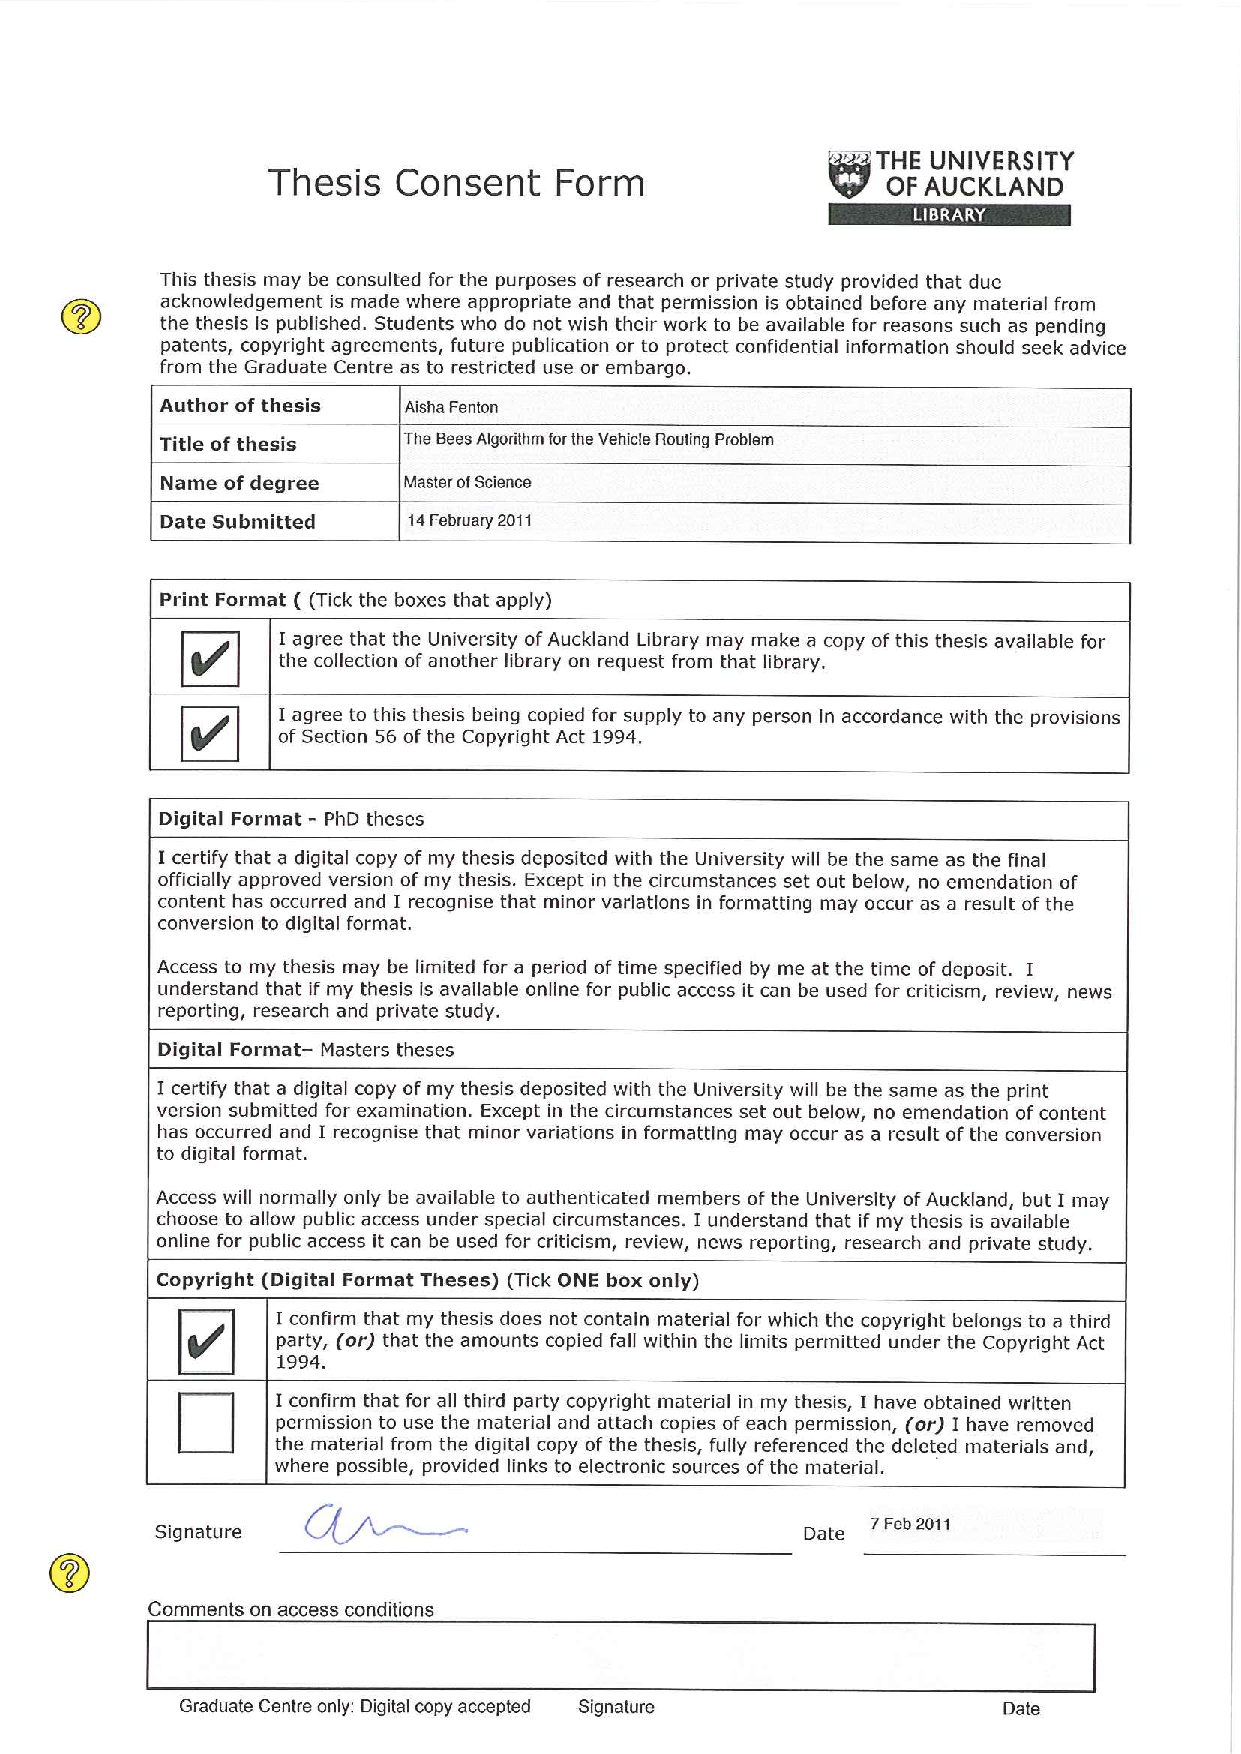
\includegraphics[angle=90, scale=0.70]{images/consent_form.pdf}

\end{document}
